%!TEX TS-program = xelatex
%!TEX encoding = UTF-8 Unicode

\documentclass[12pt]{report}
\usepackage[a4paper]{geometry} % See geometry.pdf to learn the layout options. There are lots.
\usepackage[parfill]{parskip} % Activate to begin paragraphs with an empty line \raisebox{•}{•}ather than an indent
\usepackage{graphicx,url,verbatim,setspace}
\usepackage[frenchb]{babel}
%\usepackage[Rejne]{fncychap}
\usepackage[final]{pdfpages} 
\usepackage{hyperref}
\usepackage[all]{hypcap}
\usepackage{fontspec,xltxtra,xunicode}
%\defaultfontfeatures{Mapping=tex-text}
%\setromanfont[Mapping=tex-text]{Hoefler Text}
%\setsansfont[Scale=MatchLowercase,Mapping=tex-text]{Gill Sans}
%\setmonofont[Scale=MatchLowercase]{Andale Mono}

\newcommand{\HRule}{\rule{\linewidth}{0.5mm}}

\newcommand{\blankpage}{
\newpage
\thispagestyle{empty}
\mbox{}
\newpage
}


\newcommand{\cffig}[1] {\footnote{Cf. figure~\ref{fig:#1}, p.~\pageref{fig:#1}}}

\begin{document}



\newcommand{\ladonetTitlePage}[1] {%
\begin{minipage}[t]{.5\textwidth}%
L3 Miage\\
Université de Lorraine\\
13 rue Michel Ney\\
54037 Nancy Cedex\\
~\\
Département Miage%
\end{minipage}%
\begin{minipage}[t]{.5\textwidth}%
\begin{flushright}%
{#1}
\end{flushright}%
\end{minipage}%
\vfill
\begin{center}
\HRule\\
~\\[0.4cm]
{\Huge \bfseries Conception de Systèmes \\ d' informations} \\[0.3cm]
{\Large \bfseries Conception d’une application pour un marchand spécialiste du Drive }
\\[0.4cm]
\HRule\\[1cm]
\large{Partie 1 - MCD,MCT,MOT, dictionnaire de données et les fonctionnalites}\\

\large{2014-2015}\\
\end{center}
}


\begin{titlepage}
\ladonetTitlePage{\raisebox{-.6\height}{
\includegraphics[width=1\linewidth]{ul.png}}}
\begin{center}
\vfill
\large{\textbf{Matthieu \textsc{Sahuguet}}}\\
\large{\textbf{Arthur \textsc{Mourey}}}\\
\large{\textbf{Tom \textsc{Verhoof}}}\\
\large{\textbf{Ersagun \textsc{Yalcintepe}}}\\

\vfill
\end{center}
\end{titlepage}

\blankpage



\begin{titlepage}
\ladonetTitlePage{}
\begin{center}
\vfill
\large{\textbf{Matthieu \textsc{Sahuguet}}}\\
\large{\textbf{Arthur \textsc{Mourey}}}\\
\large{\textbf{Tom \textsc{Verhoof}}}\\
\large{\textbf{Ersagun \textsc{Yalcintepe}}}\\
\vfill

\end{center}
\end{titlepage}


\begin{spacing}{1.2}

\setlength{\parskip}{16pt}

\setcounter{page}{2}

%\pagestyle{empty}
%\addtocontents{toc}{\protect\thispagestyle{empty}}
\tableofcontents

% \cleardoublepage




\chapter{Introduction}

Dans ce projet nous allons faire faire la concéption de systèmes d'information d'une application pour un marchand spécialiste du Drive et ensuite nous allons mettre en place ce SI et créer cette application. Nous allons utiliser les modèles merise pour concevoir ce SI. Pour la premiere partie, nous avons réalisé un Modèle Conceptuel des Données, avec son dictionnaire des
données ainsi qu’une liste des fonctionnalités. Comme célà sera une application web, donc nous avons décider de mettre en place cette application web via les outils web suivant :

HTML 5, CSS, JavaScript(client) et PHP (serveur).

\chapter{Modèle Conceptuel des Données}
\newpage
\centerline{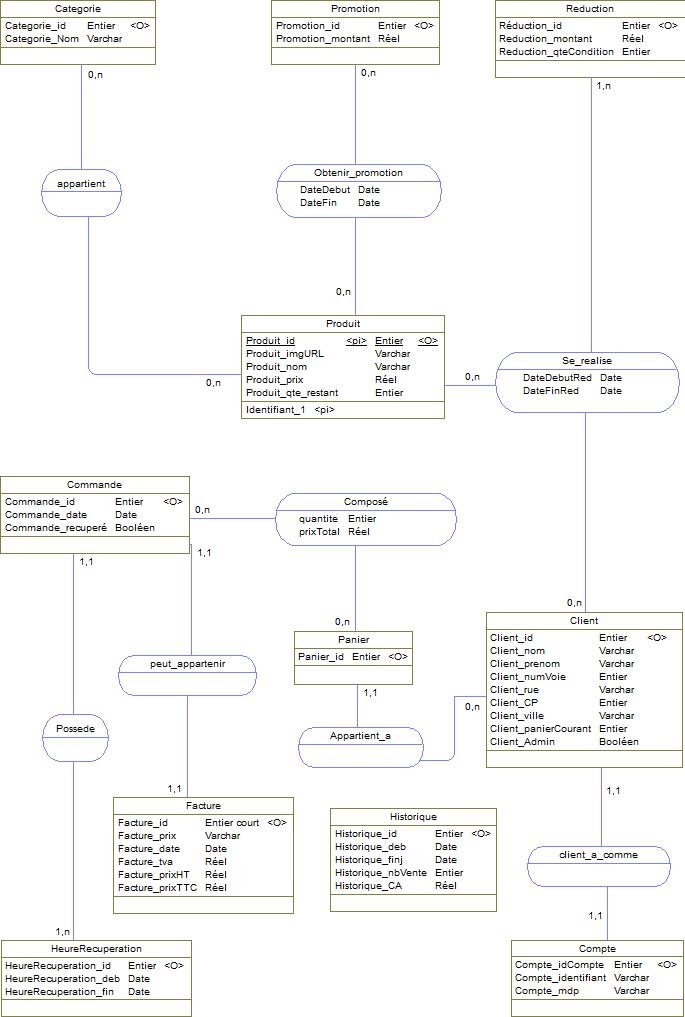
\includegraphics{mcd.jpg}}
\chapter{Dictionnaire de Données}
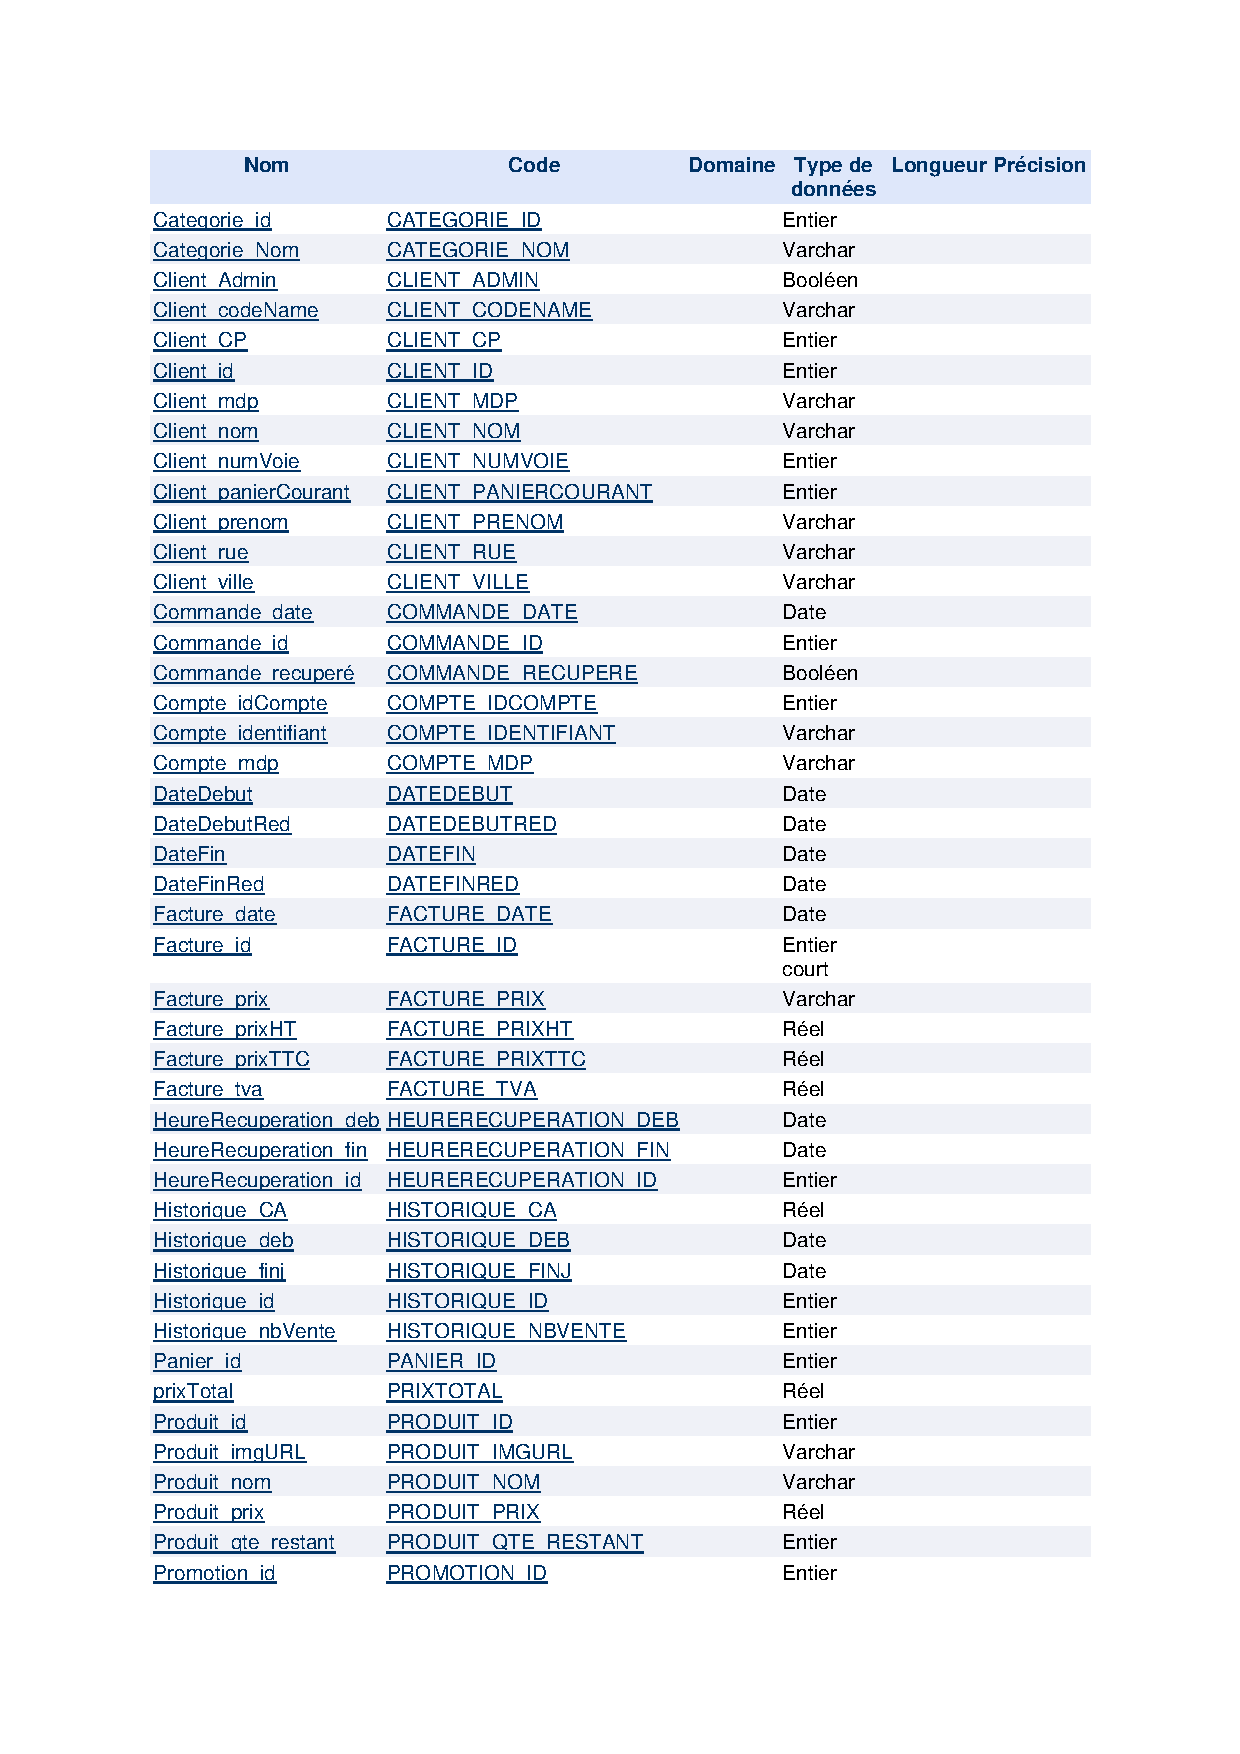
\includepdf[pages=1-1]{dict.pdf}
\chapter{Modèle Conceptuel de Traiement}
\newpage
\centerline{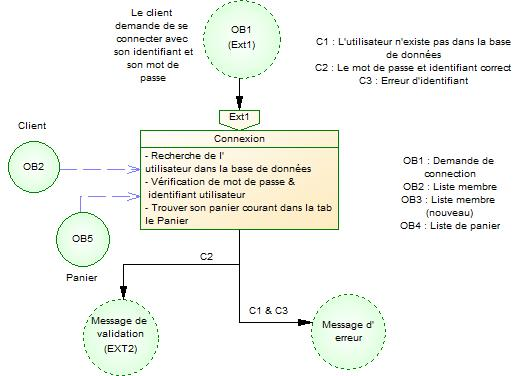
\includegraphics{mct_connexion.jpg}}
\centerline{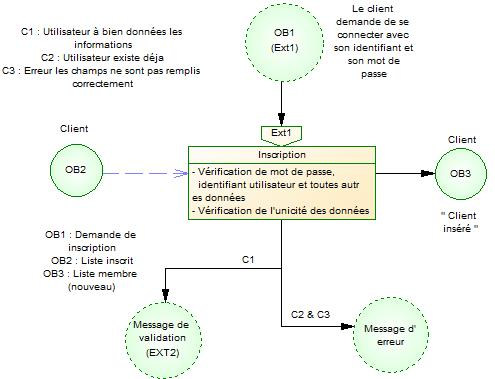
\includegraphics{mct_inscription.jpg}}
\centerline{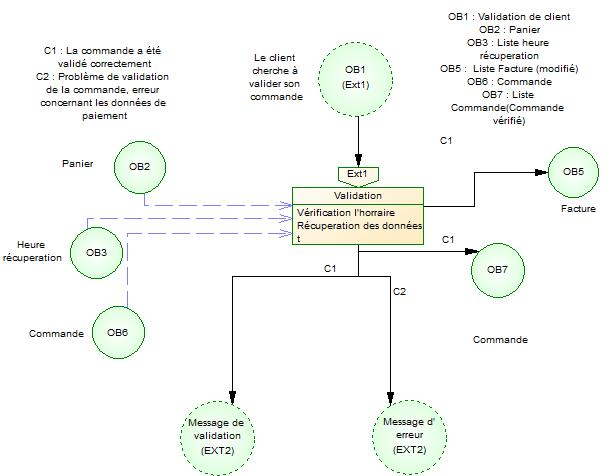
\includegraphics{mct_validationCommande.jpg}}
\centerline{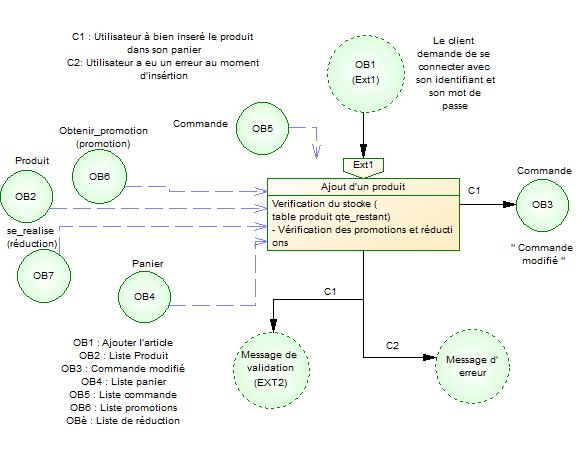
\includegraphics{mct_ajout.jpg}}
\chapter{Modèle Organisationnel de Traitement}
\newpage
\centerline{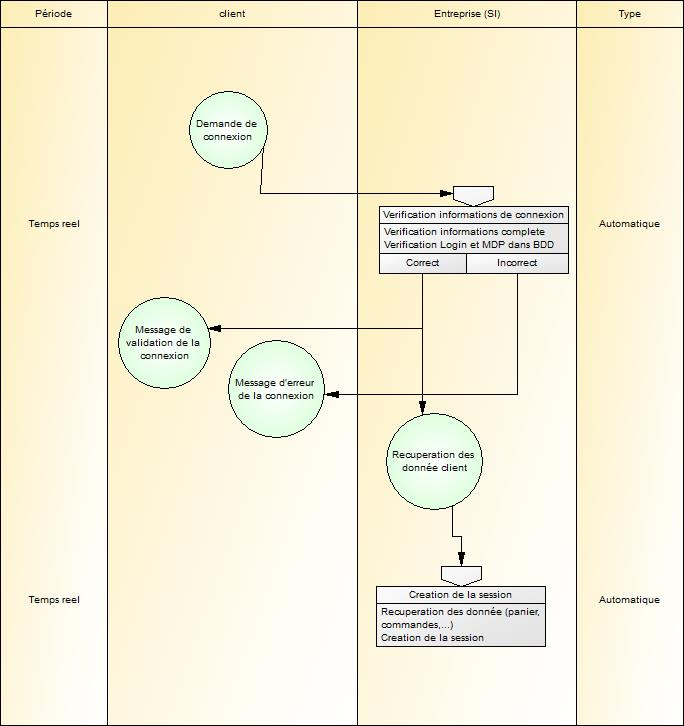
\includegraphics{mot_connexion.jpg}}
\centerline{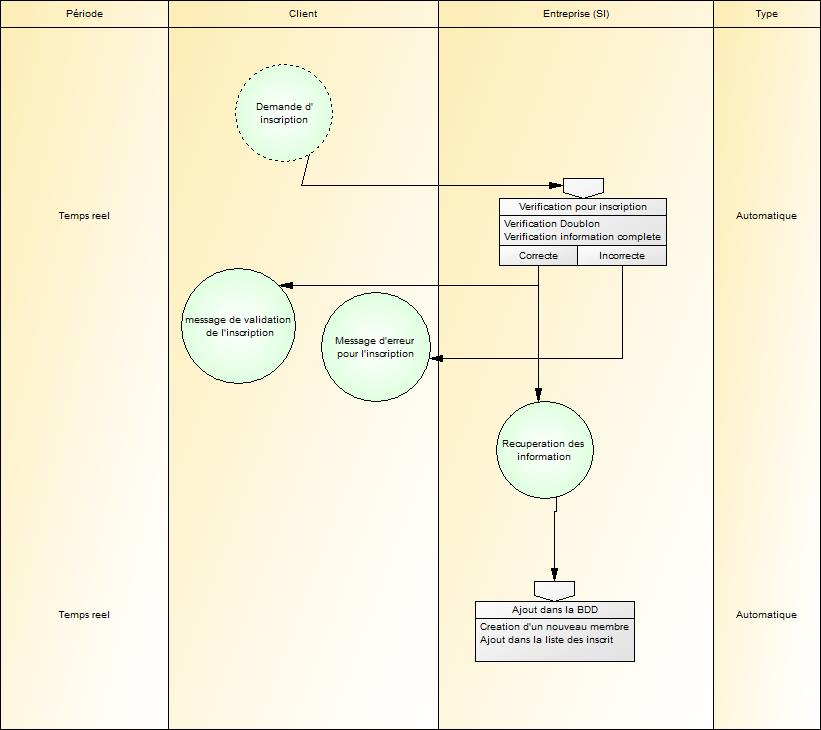
\includegraphics{mot_inscription.jpg}}
\centerline{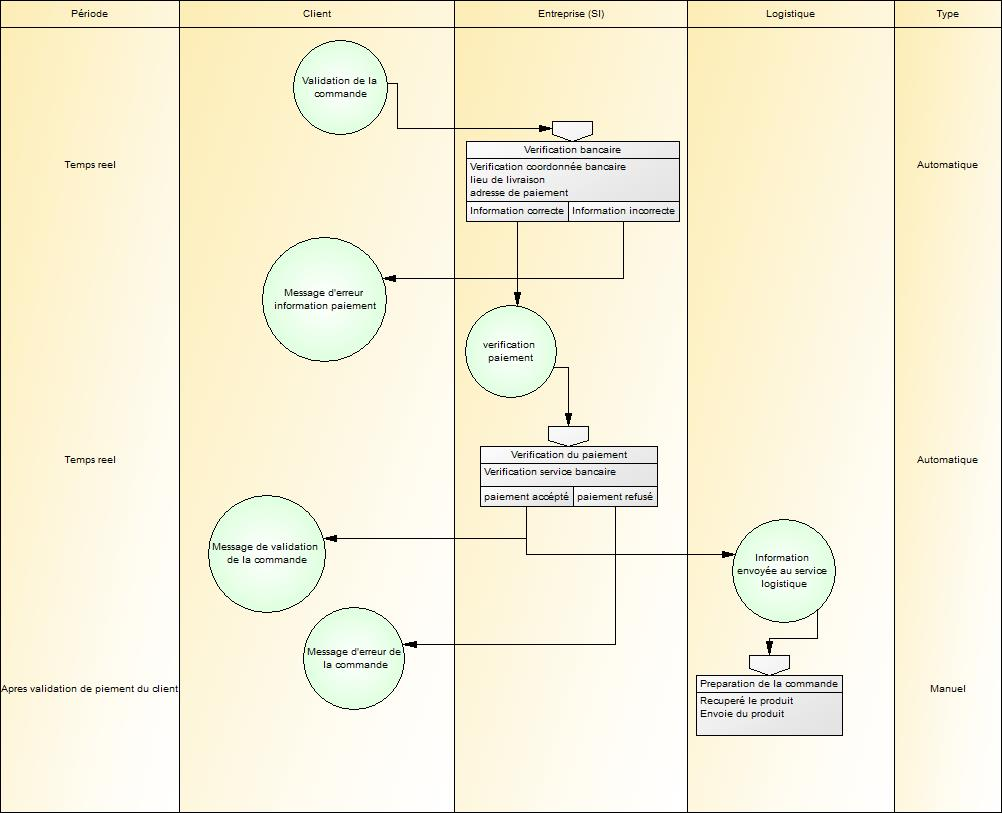
\includegraphics{mot_validationCommande.jpg}}
\centerline{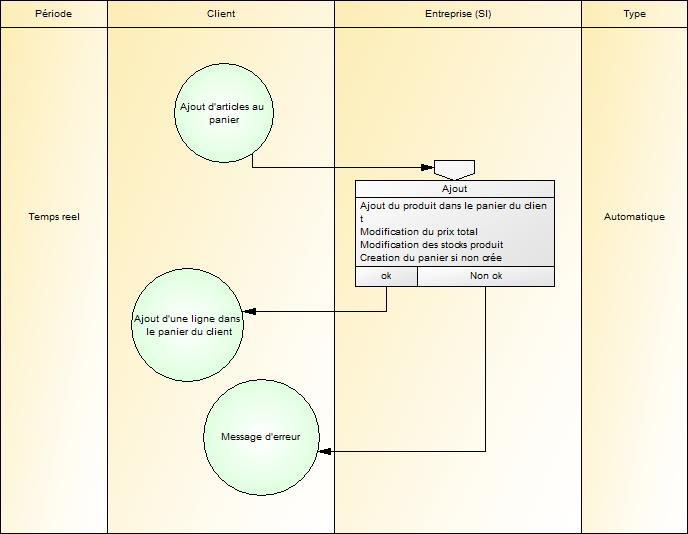
\includegraphics{mot_ajout.jpg}}
\chapter{Liste des Fonctionnalités du Site}

\section{Les fonctionnalités attendues comprennent}
\begin{itemize}

\item{La possibilité pour tout utilisateur de parcourir les différents produits}

\item{La possibilité pour l’utilisateur de filtrer/rechercher les produits par nom, par catégorie et par prix.}

\item{La possibilité pour tout utilisateur de s’inscrire, de se connecter et de se déconnecter.}

\item{Chaque client peut voir son historique des produits achetés et des commandes effectuées}

\item{L’acheteur peut remplir son panier en sélectionnant la quantité de produit désirée, ou vider un produit ou tout le contenu de son panier.}

\item{Si le panier n’est pas vide, le client verra à tout moment sur la page le contenu de son panier, le nombre de produit à l’intérieur, et le montant total.}

\item{Si le panier n’est pas vide, le client peut valider sa commande, en choisissant une date et un horaire pour retirer sa commande.}

\item{Un rappel mail sera envoyé au client une heure avant la date où il devra récupérer sa commande.}

\item{Le client peut voir la liste des offres promotionnelles et des réductions valables actuellement pour lui.}

\item{L’administrateur pourra voir un bilan journalier, hebdomadaire ou mensuel des ventes.}

\end{itemize}

\section{Les fonctionnalités attendues ne comprennent pas}
\begin{itemize}
\item{La gestion des stocks des produits, comme indiqué dans l’énoncé.}

\item{Le paiement réel, et tout ce qui est gestion des paiements, factures et retards de paiement.}

\item{La possibilité pour le client de modifier ou d’annuler sa commande une fois qu’elle a été enregistrée,
ou de redemander une date et un horaire s’il rate la livraison.}

\end{itemize}

\end{spacing}
\end{document}


